The purpose of this thesis was to categorize the dark web and visualize the result. In order to do that, the dark web had been scraped and the acquired pages had been stored in an ElasticSearch database. This was done as part of a bachelor's thesis which was being finished at the same time as this thesis. In order to retrieve the data from the database and do various operations on them, a back-end (BE) needed to be created. One of the operations was the categorization of the acquired pages. For that, an appropriate topic modeling approach was required. We chose to adopt the Latent Dirichlet Allocation (LDA). To visualize the output a graph was used. However, the data set is rather sizable and to be able to provide the user with useful information, not all pages can be displayed at once. Therefore a proper way to divide the graph into several subgraphs had to be found. We decided to use the well known Louvain algorithm (LA). To display the graph in a comprehensible manner a front-end (FE) was created.

In this chapter we will describe LDA,  which is the method used to categorize the scraped pages. Next we will talk about why it is necessary to divide immense numbers of data into clusters in order to display them as a graph. And lastly, we will detail communities and LA, the algorithm for dividing pages into communities. 

\section{Web graph} \label{webGraph}
We display our data as a graph. More precisely a web graph \cite{the_web_graph_overview}. A web graph is a graph representation of the web where nodes are portrayals of the pages and edges depict links between the pages. Web graphs tend to be built from an enormous amount of data. As such, they can  be advertised in various ways. One of the visualizations is shown in figure  \ref{hugeWebGraphFireworks}. 
\begin{figure}[ht!]
  \centering
  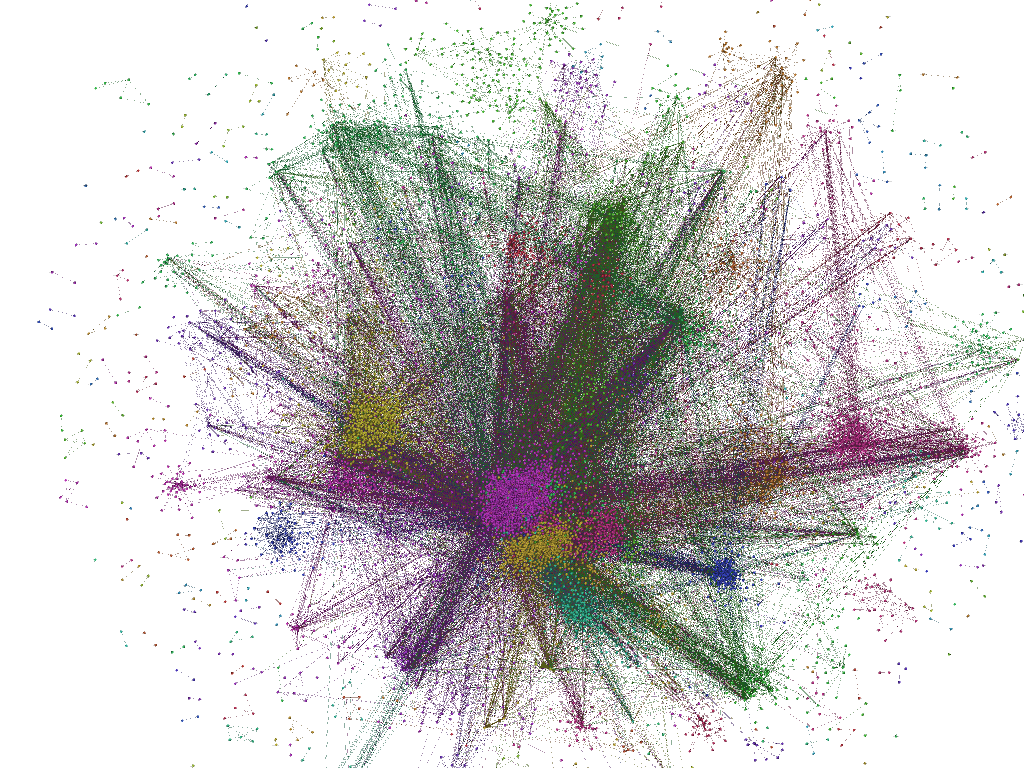
\includegraphics[width=\textwidth]{Images/hugeWebGraphFireworks.png}
  \caption{Web graph by Citeo.}
  \label{hugeWebGraphFireworks}
\end{figure} 
The web graph depicted displays all its data at once without any labels or details. The result might be useful for viewing the internet as a whole but for our purposes was insufficient since a user has had to be able to view the relationships between nodes in more detail along with information about the pages. The web graph needed to be composed of a significant smaller amount of nodes so that the view port was not too cluttered and the sought knowledge could be obtained with as little hindrances as possible. Because the majority of the nodes in the graph were not isolated \footnote{An isolated node is a node with zero incoming or outgoing edges.} we could partition the graph based on the density of its nodes, the so called communities.
\subsection{Communities}

\section{Louvain algorithm} \label{louvainAlgorithm}



